\chapter{Adapting Linicrypt to the ideal cipher model}

In this chapter, we modify the Linicrypt model to make use of the ideal cipher model instead of the random oracle model.
This means that a Linicrypt program gets access to a block cipher $\mathcal{E} = (E, D)$ where $E$ and $D$ are functions $\F \times \F \to \F$
instead of the hash function $\H : \{0,1\}^* \times \F^* \to \F$.
By the definition of a block cipher,
$\E_k := \E(k, \cdot)$ is a permutation of $\F$ for all $k \in \F$ and
$\D_k := \D(k, \cdot)$ is its inverse.
In the ideal cipher model, we assume that the block cipher has no weakness.
This is modeled by choosing each permutation $\E_k$ uniformly at random at the beginning of every security game.
We will call these programs with access to a block cipher instead of a hash function ideal cipher Linicrypt programs.

The command $y = \E(k, x)$ in an ideal cipher Linicrypt program has to be treated differently from the command $y = \H(k, x)$ when considering collision resistance,
because an attacker has access to the deterministic Linicrypt program and both directions of the block cipher $\mathcal{E} = (\E, \D)$.
Consider these two programs, $\PH$ in standard Linicrypt and $\PE$ in ideal cipher Linicrypt.

\begin{pchstack}[center,space=2cm]
  \pcbl[valign=c]{$\PH(k, x)$}{
    \pcreturn \H(k, x)
  }
  \pcbl[valign=c]{$\PE(k, x)$}{
    \pcreturn \E(k, x)
  }
\end{pchstack}
While $\PH$ is collision resistant, it is trivial to find second preimages for $\PE$
For any $k' \in \F$ the pair $(k', \D(k', \E(k, x)))$ is a second preimage to $(k,x)$.

This invertibility property of block ciphers has to be taken into account
in both the algebraic representation and the characterization of collision resistance.

\section{Algebraic representation for ideal cipher Linicrypt}

Parallel to standard Linicrypt, we will define the algebraic representation of an ideal cipher Linicrypt program.
Towards this goal, we will make the equivalent definitions to the ones in chapter \ref{chapter:revisiting_algebraic_representations}.

\begin{defn}[Ideal cipher oracle constraint]
An \textbf{ideal cipher oracle constraint} of dimension $\base$ is a tuple $(\vk, \vx, \vy)$ for
$\vk, \vx$ and $\vy$ in $\F^{1 \times \base}$.
\end{defn}

We will just say ``constraint" to mean ideal cipher oracle constraint or random oracle constraint depending on the context.

\begin{defn}[Solution of constraints]
    Let $\C$ be a set of ideal cipher constraints of dimension $\base$.
    We say a vector $\vv \in \Base$ \textbf{solves} $\C$ if
    $\vy \vv = \E(\vk \vv, \vx \vv)$ for all $(\vk, \vx, \vy) \in \C$.
    Such a $\vv$ is also called a \textbf{solution} of $\C$.
    The set of all solutions to $\C$ is called $\sol(\C)$.
\end{defn}

Let $\P$ be an ideal cipher Linicrypt program.
Base variables and associated vectors are defined exactly as defined in standard Linicrypt.
The only difference is that the base variables can now be instantiated with calls to the ideal cipher instead of calls to the random oracle.
For each command in $\P$ of the form $v_3 = \E(v_1,v_2)$
we define the \textbf{associated ideal cipher constraint} $(\vv_1, \vv_2, \vv_3)$.
Note, that the bold variant of the intermediate variable denotes its associated vector.
Correspondingly, each query to $\D$ of the form $v_3 = \D(v_1,v_2)$,
is associated with the constraint $(\vv_1, \vv_3, \vv_2)$.
We call the set of all associated constraints $\C$. 
The input matrix $\I$ and output matrix $\O$ are defined in the same way as in standard Linicrypt.
We call $(\I,\O,\C)$ the algebraic representation of $\P$.
Then, the following statement holds true, which is the trivial direction of Corollary \ref{det_solvable_equiv} in standard Linicrypt.

\begin{lemma}
    Let $\P$ be an ideal cipher Linicrypt program with algebraic representation $(\I,\O,\C)$.
    Let $\vv$ denote the values of the base variables in an execution of $\P$ with input $(\dts i k)$ and output $(\dts o l)$.
    Then $\vv$ is a solution to $\C$ with $\I\vv = (\dts i k)$ and $\O\vv = (\dts o l)$
\end{lemma}

\begin{proof}
    The statements $\I\vv = (\dts i k)$ and $\O\vv = (\dts o l)$ follow from definition as in standard Linicrypt.
    Each constraint in $\C$ comes from a command in $\P$ with a query to the ideal cipher.

    Take some $(\vk, \vx, \vy) \in \C$.
    After renaming the intermediate variables of $\P$,
    it is associated either to the command $y = \E(k, x)$ or to the command $x = \D(k, y)$.
    In the first case we have $\vy\vv = y = \E(k, x) = \E(\vk\vv, \vx\vv)$.
    In the second case we also have $y = \E(k,x)$
    by the properties of the ideal cipher $\mathcal{E} = (\E,\D)$.
    Therefore, $\vv$ is a solution to $\C$.
\end{proof}

The main definition that changes with ideal cipher Linicrypt is the one determining if $\C$ is deterministically solvable.
This definition captures the properties of the black box that $\P$ and an attacker can access.
In standard Linicrypt the black box is a one-way random function.
In ideal cipher Linicrypt the black box is a random permutation that can be computed both ways,
as both the Linicrypt program and the attacker have full access to the ideal cipher $\mathcal{E} = (\E,\D)$.

To simplify the notation we extend the linear algebra operators $\rowsp$ and $\ker$
to be able to use them naturally with constraints and sets of constraints.
We define for a constraint $c = (\vk, \vx, \vy)$:
\begin{align*}
\rowsp(c) &= \rowsp(\vk) + \rowsp(\vx) + \rowsp(\vy) \\
\ker(c) &= \ker(\vk) \cap \ker(\vx) \cap \ker(\vy)
\end{align*}
For a set of constraints $\C$ we write:
\begin{align*}
\rowsp(\C) &= \sum_{c \, \in \, \C} \rowsp(c) \\
\ker(\C) &= \bigcap_{c \, \in \, \C} \ker(c)
\end{align*}

\begin{defn}[Deterministically Solvable]
\label{def_det_solvable_ic}
    Let $\C$ be a finite well-defined set of ideal cipher constraints of dimension $\base$,
    and let $\I \in \F^{k \times \base}$ for some $k \in \NN$.
    $\C$ is \textbf{deterministically solvable fixing} $\I$ (or fixing $\rowsp(\I)$)
    if there exists an ordering $(c_1, \dots, c_n)$ of $\C$
    such that for all $i=1, \dots, n$ the following holds.
    
    Let the components of $c_i$ be called $(\vk_i, \vx_i, \vy_i)$.
    One can write either
    % \vspace{-2mm}
    % \begin{equation*}
    % \textrm{(case a) } \Q_i = \m{\vk_i \\ \vx_i} \textrm{ and } \va_i = \vy_i 
    % \textrm{ or (case b) } \Q_i = \m{\vk_i \\ \vy_i} \textrm{ and } \va_i = \vx_i,
    % \end{equation*}
    \vspace{-4mm}
    \begin{center}
    $\Q_i = \m{\vk_i \\ \vx_i}$ and $\va_i = \vy_i$ (Case a) \,or\,
    $\Q_i = \m{\vk_i \\ \vy_i}$ and $\va_i = \vx_i$ (Case b),
    \end{center}
    \vspace{-4mm}
    such that:
    
    % We destructure $c_i$ into $(\vk_i, \vx_i, \vy_i)$.
    % Then one can write either $\Q_i = \m{\vk_i \\ \vx_i}$ and $\va_i = \vy_i$ (case a)
    % or $\Q_i = \m{\vk_i \\ \vy_i}$ and $\va_i = \vx_i$ (case b) such that:
    \begin{enumerate}
    \item
        \label{solvable1_ic}
        $\rows(\Q_i) \subseteq \rowsp(\I) + \rowsp(\dts \va {i-1} )$
    \item
        \label{solvable2_ic}
        $\va_i \notin \rowsp(\I) + \rowsp(\dts \va {i-1} )$
    \end{enumerate}
    Additionally we require that $\rows(\I) \cup \{\va_1, \dots, \va_n\}$ form a basis of $\F^{1\times\base}$.
    We call $(c_1, \dots, c_n)$ a solution ordering of $\C$ fixing $\I$ (or fixing $\rows(\I)$).
\end{defn}

Note that the case distinction (Case a and Case b) is what models the invertibility of the ideal cipher.
It is indeed an exclusive ``or"
because condition 1.~of Case a implies that condition 2.~of Case b is false.
With these definitions in place, the Lemmas from Chapter \ref{chapter:revisiting_algebraic_representations} can be formulated in the same way.

\begin{lemma}
\label{alg_rep_det_solvable_ic}
    Let $(\I, \O, \C)$ be the algebraic representation of a deterministic ideal cipher Linicrypt program $\P$ taking $k$ inputs.
    Then $\C$ is deterministically solvable fixing $\I$.
\end{lemma}

\begin{sketch}
    For each constraint $c = (\vk, \vx, \vy)$ in $\C$ we set $\Q = \m{\vk^\top & \vx^\top}^\top$ and $\va = \vy$ if $c$ is associated to a call to $\E$.
    If $c$ is associated to a call to $\D$,
    we set $\Q = \m{\vk^\top & \vy^\top}^\top$ and $\va = \vx$.
    The rest of the proof is identical to the proof of Lemma \ref{alg_rep_det_solvable}.
\end{sketch}

\begin{lemma}
\label{is_algebraic_repr_ic}
    Let $\C$ be a finite well-defined set of ideal cipher constraints of dimension $\base$ with $|\C| = n$,
    let $\I = \m{\Id_k & 0} \in \F^{k\times\base}$ for $k = \base - n$
    and let $\O \in \F^{l \times \base}$ for some $l \in \NN$.
       
    $(\I, \O, \C)$ is the algebraic representation of a deterministic ideal cipher Linicrypt program $\P$
    if there exists an ordering $(c_1, \dots, c_n)$ of $\C$
    such that for all $i=1, \dots, n$ one of the following cases hold for $(\vk_i, \vx_i, \vy_i) = c_i$:
    \begin{enumerate}[label=(\alph*)]
    \item
    $\vy_i = \ve_{k+i}$ and $\{\vk_i, \vx_i\} \subseteq \spn(\dts \ve {k+i-1})$ or
    \item
    $\vx_i = \ve_{k+i}$ and $\{\vk_i, \vy_i\} \subseteq \spn(\dts \ve {k+i-1})$
    \end{enumerate}
\end{lemma}

\begin{sketch}
    The proof idea is the same as for Lemma \ref{is_algebraic_repr}.
    The $k$ inputs are handled as in standard Linicrypt.
    Consider the constraint $c_i$.
    If case (a) holds, then we convert this constraint into a command of the form $v_{k+i} = \E(q_1, q_2)$,
    for $q_1$ and $q_2$ being intermediate variables created by a linear combination.
    Then condition $\{\vk_i, \vx_i\} \subseteq \spn(\dts \ve {k+i-1})$ ensures that these linear combinations are well-defined.
    As $\base = k + n$, all base variables have been set after $n$ query commands.
    We can use the rows of $\O$ to define the Linicrypt commands for the output variables.
\end{sketch}

\begin{lemma}
\label{det_solvable_lemma_ic}
    Let $\C$ be a set of deterministically solvable constraints fixing $\Inp \in \F^{k \times \base}$ for some $k \in \NN$.
    Let $\O \in \F^{\out \times \base}$ be an arbitrary output matrix for some $\out \in \NN$.
    Then there is a basis change $\B \in \F^{\base \times \base}$
    and a Linicrypt program $\P$,
    such that $(\Inp \B, \O \B, \C \B)$ is its algebraic representation.
\end{lemma}

\begin{sketch}
    By setting $\Q_i$ and $\va_i$ as in the definition \ref{def_det_solvable_ic} we can copy the proof of Lemma \ref{det_solvable_lemma}.
\end{sketch}

\begin{lemma}
\label{lemma:solution_space_bijection_ic}
    Let $\C$ be deterministically solvable fixing some $\I$.
    If we view $\I$ as a function $\Fsp \to \F^k$,
    then $\I|_{\sol(\C)}$ is a bijection.
\end{lemma}

\begin{sketch}
    By setting $\Q_i$ and $\va_i$ as in the definition \ref{def_det_solvable_ic} we can copy the proof of Lemma \ref{lemma:solution_space_bijection}.
\end{sketch}

\begin{corollary}
\label{corollary:det_solvable_computeable_ic}
    Let $\C$ be deterministically solvable fixing some $\I$.
    For each element in $\F^k$ its inverse under $\I|_{\sol(\C)}$ can be computed with $|\C|$ queries to the ideal cipher.
\end{corollary}

\begin{sketch}
    The proof is identical to the proof of Corollary \ref{det_solvable_computeable}.
\end{sketch}

\section{Collision Structure}

We have all the prerequisites to prove the analog of Lemma \ref{collision_structure_implies_attack}.
That is, we can give a sufficient condition for a program to be susceptible to a constant time second preimage attack.

\begin{prop}
\label{collision_structure_implies_attack_ic}
    Let $\P = (\I, \O, \C)$ be a deterministic ideal cipher Linicrypt program.
    Assume we can write $\C = \Ccs \sqcup \Cfix$ and
    $\Ccs$ is deterministically solvable fixing some $\Ics$ such that
    \begin{equation}
    \label{cs_condition_ic}
        \rowsp(\Ics) \supsetneq \rowsp(\O) + \rowsp(\Cfix).
    \end{equation}
    Then an attacker can find second preimages with $|\Ccs|$ queries.
    We say a program has a collision structure if it fulfills condition \eqref{cs_condition_ic}.
\end{prop}

Here we will give a more formal proof of this statement.
\begin{proof}
    The proof describes how to find a second preimage to some input $(\dts i k)$ to $\P$.
    By executing $\P$ on $(\dts i k)$ we compute the values of the base variables $\vv \in \sol(\C)$.
    Recall the bijection $\Ics|_{\sol(\Ccs)}: \sol(\Ccs) \to \F^{k'}$ where $k'$ is the number of rows of $\Ics$. 
    Instead of seeing this bijection as a map into the input space of $\P$, we will see it as a map into the quotient space
    $\sfrac{\Fsp}{\ker(\Ics)}$.
    This quotient space is defined by the equivalence relation $\vv \; \simcs \; \vw \iff \vv - \vw \in \ker(\Ics)$.
    We denote it by:
    \begin{align*}
    \widetilde\Ics: \sol(\Ccs) &\to \bigslant{\Fsp}{\ker(\Ics)} \\
    \vv &\mapsto [\vv]_\simcs
    \end{align*}
    
    Using condition \eqref{cs_condition_ic} we will map
    $\sfrac{\Fsp}{\ker(\Ics)}$ to $\sfrac{\Fsp}{\big(\ker(\O) \cap \ker(\Cfix)\big)}$
    non injectively.
    First we rewrite the condition \eqref{cs_condition_ic}:
    \begin{align}
    \eqref{cs_condition_ic} &\iff \ker(\Ics)^\top \supsetneq \ker(\O)^\top + \ker(\Cfix)^\top \\
    &\iff \ker(\Ics)^\top \supsetneq \big(\ker(\O) \cap \ker(\Cfix)\big)^\top \\
    \label{cs_kernel_ic}
    &\iff \ker(\Ics) \subsetneq \ker(\O) \cap \ker(\Cfix)
    \end{align}
    Let $\simfix$ denote the equivalence relation defining the quotient $\sfrac{\Fsp}{(\ker(\O) \cap \ker(\Cfix))}$.
    Consider the map
    \begin{align*}
        \lambda: \bigslant{\Fsp}{\ker(\Ics)} &\to \bigslant{\Fsp}{\big(\ker(\O) \cap \ker(\Cfix)\big)} \\
        [\vv]_{\simcs} &\mapsto [\vv]_{\sim_{fix}}.
    \end{align*}
    To show that it is well-defined,
    we need to show that it is independent of the chosen representative.
    Let $[\vv]_\simcs = [\vw]_\simcs$ for arbitrary $\vv,\vw \in \Fsp$.
    By definition $\vv-\vw \in \ker(\Ics)$.
    Using $\eqref{cs_kernel_ic}$ we have $[\vv]_\simfix = [\vw]_\simfix$.
    Now we show that $\lambda$ is not injective.
    Let $\vw \in \ker(\O) \cap \ker(\Cfix)$ but $\vw \notin \ker(\Ics)$,
    so $[\vv + \vw]_\simcs \neq [\vv]_\simcs$.
    This is possible because by \eqref{cs_kernel_ic} $\ker(\Ics)$ is strictly smaller than $\ker(\O) \cap \ker(\Cfix)$.
    Then
    \[
        \lambda([\vv + \vw]_\simcs) = [\vv + \vw]_\simfix = [\vv]_\simfix = \lambda([\vv]_\simcs).
    \]
    As a consequence the concatenation $\lambda \circ \widetilde\Ics$ is not injective.
    Therefore, we can find a $\vv' \in \sol(\Ccs)$ with $\vv' \neq \vv$ such that $[\vv']_\simfix = [\vv]_\simfix$.
    The latter is equivalent to $\O\vv' = \O\vv$ and $\vv' - \vv \in \ker(c)$ for all $c \in \Cfix$.
    As $\vv$ is a solution to $\Cfix$ it follows that $\vv'$ is a solution, too.
    Summing up, $\vv' \in \sol(\Ccs) \cap \sol(\Cfix) = \sol(\C)$ and $\vv' \neq \vv$.
    
    By the bijection argument, we know that $\I\vv' \neq \I\vv$ and hence
    $\I\vv'$ is a second preimage to $\I\vv = (\dts i k)$.
    
    We argue why the second preimage is computable with $|\Ccs|$ queries.
    To compute such a $\vv'$ we need to compute preimages of $\lambda \circ \widetilde\Ics$.
    Because $\lambda$ is just a linear map, the space of preimages to any element in its image can be computed without any queries to $\H$.
    We can choose a preimage $[\vv']_\simcs$ to $[\vv]_\simfix$ from its space of preimages arbitrarily while making sure that $[\vv']_\simcs \neq [\vv]_\simcs$.
    The inverse of the bijection $\widetilde\Ics$ is computable with $|\Ccs|$ queries by Corollary \ref{corollary:det_solvable_computeable_ic}.
\end{proof}

We give an example of a program that has a collision structure due to the invertibility of $\E$.

\begin{pchstack}[center, space=2cm]
    \pcbl[valign=c]{$\PE[col](a,b,c)$}{
        k_1 = c \\
        x_1 = b \\
        y_1 = \E(k_1, x_1) \\
        k_2 = a \\
        x_2 = y_1 \\
        y_2 = \E(k_2, x_2) \\
        \pcreturn y_1 + y_2
    }
    \pcbm[valign=c]{Algebraic Representation}{
    \begin{pcmbox}
        \arraycolsep=3pt
        \begin{array}{r wl{3mm} l}
        \O    = \> \begin{bmatrix}0 \> 0 \> 0 \> 1 \> 1\end{bmatrix} \\[2pt]
        \vk_1 = \> \begin{bmatrix}0 \> 0 \> 1 \> 0 \> 0\end{bmatrix} \\[2pt]
        \vx_1 = \> \begin{bmatrix}0 \> 1 \> 0 \> 0 \> 0\end{bmatrix} \\[2pt]
        \vy_1 = \> \begin{bmatrix}0 \> 0 \> 0 \> 1 \> 0\end{bmatrix} \\[2pt]
        \vk_2 = \> \begin{bmatrix}1 \> 0 \> 0 \> 0 \> 0\end{bmatrix} \\[2pt]
        \vx_2 = \> \begin{bmatrix}0 \> 0 \> 0 \> 1 \> 0\end{bmatrix} \\[2pt]
        \vy_2 = \> \begin{bmatrix}0 \> 0 \> 0 \> 0 \> 1\end{bmatrix} 
        \end{array}
    \end{pcmbox}
    }
\end{pchstack}

We can set $\Ccs = \{c_1\}$, $\Cfix = \{c_2\}$ and $\Ics = \m{\O \\ \vk_2 \\ \vx_2 \\ \vk_1}$.

Then $\rowsp(\Ics) = \big( \rowsp(\O) + \rowsp(\Cfix) \big) \oplus \rowsp(\vk_1)$, so condition \eqref{cs_condition_ic} is fulfilled.
$\Ccs$ is deterministically solvable fixing $\Ics$.
We can set $\Q_1 = \m{\vk_1 \\ \vy_1}$ and $\va_1 = \vx_1$, and then we have: 
\begin{enumerate}
    \item $\rows(\Q_1) \subseteq \rowsp(\Ics)$
    \item $\va_1 \notin \rowsp(\Ics)$
\end{enumerate}

This makes Lemma \ref{collision_structure_implies_attack_ic} applicable and the Lemma describes how to construct an attack in the form of a Linicrypt program.

In plain language,
we can fix the output, set the second query and answer to the same values as for the given preimage and choose $k_1$ arbitrarily.
This determines the key $k_1$ and answer $y_1$ of the first query to $\E$, but not the query itself.
By using $\D$ we get the unique corresponding query $x_1$.
Then $(k_2, x_1, k_1)$ is a second preimage.

Now will work towards the converse of this statement.
That is, we are trying to answer the question:
If $\P$ doesn't have a collision structure,
is it collision resistant?
We will confirm this for the case of a Linicrypt program which makes only a single query to the ideal cipher.

\begin{defn}
    A set of ideal cipher constraints $\C$ is called unsolvable fixing a space $\Fix \subseteq \Frowsp$ if for every ordering $(\dts c n)$ of $\C$,
    we have some $c_i = (\vk_i, \vx_i, \vy_i)$ such that both
    \begin{enumerate}
    \item    $\vy \in \Fix + \rowsp(\{\dts c {i-1}\}) + \rowsp(\vk, \vx)$ and
    \item    $\vx \in \Fix + \rowsp(\{\dts c {i-1}\}) + \rowsp(\vk, \vy)$.
    \end{enumerate}
\end{defn}

\begin{lemma}
\label{lemma_no_collision_structure}
    If $\P = (\I,\O,\C)$ does not have a collision structure,
    then for every split $\C = \Ccs \sqcup \Cfix$ we have one of the following:
    \begin{enumerate}
    \item $\Ccs$ is deterministically solvable fixing $\rowsp(\O) + \rowsp(\Cfix)$
    \item $\Ccs$ is unsolvable fixing $\rowsp(\O) + \rowsp(\Cfix)$
    \end{enumerate}
\end{lemma}

\begin{proof}
    Assume $\P$ does not have a collision structure.
    Let $\C = \Ccs \sqcup \Cfix$ be an arbitrary split of the set of constraints.
    Then for any matrix $\Ics$ with $\rowsp(\Ics) \supsetneq \rowsp(\O) + \rowsp(\Cfix)$ we have
    $\Ccs$ is not deterministically solvable fixing $\Ics$.
    We now assume condition \textit{2.}~from Lemma \ref{lemma_no_collision_structure} not true
    and show that this implies \textit{1.}~from Lemma \ref{lemma_no_collision_structure} is true.
    So we assume $\Ccs$ is not unsolvable fixing $\Fix = \rowsp(\O) + \rowsp(\Cfix)$.
    Then there is an ordering $(c_1, \dots, c_n)$ of $\Ccs$ such that for every $i$ we have
    $\vy \notin \Fix + \rowsp(\{\dts c {i-1}\}) + \rowsp(\{ \vk, \vx \})$ or
    $\vx \notin \Fix + \rowsp(\{\dts c {i-1}\}) + \rowsp(\{ \vk, \vy \})$.
    This gives the condition \textit{2.}~of the definition of deterministically solvable.
    Hence, we can add some dimensions to $\Fix$ and call it $\Fix' \supset \Fix$ such that
    $\Ccs$ is deterministically solvable fixing $\Fix'$.
    But if $\Fix' \supsetneq \Fix$ this would contradict the assumption that $\P$ does not have a collision structure.
    Therefore, we know that $\Ccs$ is deterministically solvable fixing $\Fix = \rowsp(\O) + \rowsp(\Cfix)$.
\end{proof}

\begin{corollary}
\label{corollary:single_query_properties}
    Let $\P = (\I, \O, \C)$ be a program making only a single call to the ideal cipher.
    Then $\C = \{ (\vk, \vx, \vy)\}$ for some $\vk, \vx, \vy \in \Frowsp$.
    Assume $\P$ does not have a collision structure but there exists $\vv \neq \vv'$ in $\sol(\C)$ with $\O\vv = \O\vv'$.
    Then the following hold:
    \begin{enumerate}
    \item $\ker(\O) \cap \ker(\C) = \{0\}$
    \item $\vy \in \rowsp(\O) + \rowsp(\vk, \vx)$
    \item $\vx \in \rowsp(\O) + \rowsp(\vk, \vy)$
    \end{enumerate}
\end{corollary}
\begin{proof}
    If we set $\Ccs = \{\}$ then case \textit{2.}~from Lemma \ref{lemma_no_collision_structure} cannot be true.
    Because $\{\}$ is deterministically solvable fixing $\rowsp(\O) + \rowsp(\C)$ we have a bijection between
    $\sol(\{\}) = \Fsp$ and $\rowsp(\O) + \rowsp(\C)$.
    Because $\rowsp(\O) = \ker(\O)^\perp$ and $\rowsp(\C) = \ker(\C)^\perp$
    this implies $\ker(\O) \cap \ker(\C) = \{0\}$.
    
    If we set $\Ccs = \C$ on the other hand,
    then case \textit{1.}~from Lemma \ref{lemma_no_collision_structure} cannot be true.
    This is because if it was, then there wouldn't exist vectors $\vv \neq \vv'$ in $\sol(\C)$ with $\O\vv = \O\vv'$.
    Therefore, $\C$ is unsolvable fixing $\rowsp(\O)$ which gives exactly 
    $\vy \in \rowsp(\O) + \rowsp(\{\vk, \vx\})$ and
    $\vx \in \rowsp(\O) + \rowsp(\{\vk, \vy\})$.
\end{proof}

Let us first state a small mathematical Lemma wich serves to simplify the bounds on the advantages without giving away too much.
\begin{lemma}
\label{lemma:fraction_bound}
    Let $a,b,c$ be in $\RR_+$ with $a,b > c$. Then
    \[
    \frac{a-c}{b-c} \leq \frac{a}{b} \iff a \leq b.
    \]
\end{lemma}
We give a short proof of this statement.
\begin{proof}
    Assume $a,b,c$ fulfill the stated conditions.
    Then we can write the following sequence of equivalent statements:
    \begin{align*}
         & \frac{a-c}{b-c} \leq \frac{a}{b} \\
        \iff& \log(a-c) - \log(b-c) \leq \log(a) - \log(b) \\
        \iff& \log(b) - \log(b-c) \leq \log(a) - \log(a-c) \\
        \iff& \log(b) - \log(b-c) \leq \log(a) - \log(a-c) \\
        \iff& a \leq b
    \end{align*}
    The last equivalence follows from the derivative of the logarithm being monotonically decreasing.
\end{proof}

\begin{prop}
\label{prop:single_query_cr_resistance}
    Let $\P = (\I, \O, \C)$ be a program making only a single call to the ideal cipher,
    i.e. $\C = \{ (\vk, \vx, \vy)\}$ for some $\vk, \vx, \vy \in \Frowsp$.
    Assume there is an adversary $\adv$ making $N$ queries to the ideal cipher winning the collision resistance security game with
    \[
        \cradv{\A, \P} > \frac{(N+1)N}{2|\F|}
        % \prob{\mathsf{ColGame}(\P, \adv, \lambda) = 1 } > \frac{N(N-1)}{2(|\F| - N)}.
    \]
    Then $\P$ has a collision structure.
\end{prop}

This proof is based on the proofs from McQuoid, Swope and Rosulek in \cite[Lemma 10]{TCC:McQSwoRos19} and from Boneh-Shoup in \cite[Theorem 8.4 (Davies-Meyer)]{Boneh2015CourseIA}.

\begin{proof}
    Assume towards a contradiction that there is such an adversary $\A$ making $N$ queries
    and that $\P$ does not have a collision structure.
    % Without loss of generality we can assume that $\A$ has made the queries to the ideal cipher
    % can output the whole tuple of base variables $\vv$ and $\vv'$ for a collision. 
    We will work with the transcript between the adversary and the ideal cipher.
    Let $\mathcal{T}: \{1, \dots, N\} \to \F^3$ be the function defined by $\mathcal{T}(i) = (k, x, y)$,
    if the $i$th query of $\A$ is $\E(k, x)$ with response $y$ or if it is $\D(k, y)$ with response $x$.

    Let $\v i$ and $\v i'$ be the output of $\A$ in the event that it successfully found a collision.
    As $\C$ is deterministically solvable fixing $\I$, they correspond to unique vectors $\vv \neq \vv'$ in $\sol(\C)$.
    We can assume the adversary actually makes the queries corresponding to these inputs,
    therefore $(\vk \vv, \vx \vv, \vy \vv)$ and $(\vk \vv', \vx \vv', \vy \vv')$ are contained in $\im(\mathcal{T})$.
    Otherwise, the adversary has won just by chance.
    If we assume $N \geq 2$, the probability for this event is bounded from above by
    \[
        \frac{1}{|\F| - N} \leq \frac{(N+1)N - 2N}{2|\F| - 2N} \leq \frac{(N+1)N}{2|\F|}.
    \]
    This would contradict the assumption in the Lemma.

    Let $i$ and $j$ be defined by $\mathcal{T}(i) = (\vk \vv, \vx \vv, \vy \vv)$
    and $\mathcal{T}(j) = (\vk \vv', \vx \vv', \vy \vv')$. 
    That is, at query $i$ the adversary has determined the values involved in the query for $\P(\v i)$ and
    at query $j$ it has determined the values involved in the query for $\P(\v i')$.
    
    Consider the case $i = j$.
    This means $\vv - \vv \in \ker(\C)$.
    By assumption $\v i$ and $\v i'$ are collisions, so $\vv - \vv' \in \ker(\O)$.
    Corollary \ref{corollary:single_query_properties} states $\ker(\O) \cap \ker(\C) = \{0\}$,
    so $\vv = \vv'$. 
    This is a contradiction to $\v i \neq \v i'$.
    
    Therefore, we have $i \neq j$.
    By modifying $\A$,
    we can assume it outputs the value it fixes first as its first output.
    Because $i$ corresponds $\vi$ and $j$ to $\vi'$, we have $i < j$.
    Consider the point where $\A$ sent its $j$th query and is waiting to receive the answer from the ideal cipher.
    If this query was to $\E$ we define $\Q = \m{\vk \\ \vx}$ and $\va = \vy$,
    otherwise we define $\Q = \m{\vk \\ \vy}$ and $\va = \vx$.
    
    In either case, we know from Corollary \ref{corollary:single_query_properties} that
    \begin{equation}
    \label{security_proof_equation}
    \va \in \rowsp(\O) + \rowsp(\Q) ,\quad \textrm{which means} \quad \va = \v \lambda \O + \v \gamma \Q.
    \end{equation}
    At query $j$ the vectors $\Q\vv, \va\vv, \Q\vv'$ and $\O(\vv' - \vv)$ are determined.
    The latter is equal to $0$ by the assumption that $\v i$ and $\v i'$ are a collision.
    Therefore, we can use \eqref{security_proof_equation} to show
    \begin{equation*}
    \va (\vv' - \vv) = \v\lambda\O(\vv' - \vv) + \v\gamma \Q (\vv' - \vv),
    \end{equation*}
    which is equivalent to
    \begin{equation}
    \label{security_proof_equation2}
    \va \vv' = \va\vv + \v\gamma \Q \vv' - \v\gamma \Q\vv.
    \end{equation}
    All the values on the right of \eqref{security_proof_equation2} have been determined,
    while $\va\vv'$ is sampled uniformly from a set of size at least $|\F| - j + 1$.
    We call the event that equation \eqref{security_proof_equation2} holds $Z_{ij}$, so
    \[
        \prob{Z_{ij}} = \frac{1}{|\F| - j + 1}.
    \]
    Using the union bound we get
    \begin{equation*}
    \cradv{\A, \P}
    \leq \sum_{j=1}^{N} \sum_{i=1}^{j-1} \prob{Z_{ij}}
    \leq \sum_{j=0}^{N-1} \frac{j}{|\F| - j}
    \leq \frac{(N-1)N}{2(|\F| - N)}
    \leq \frac{(N+1)N}{2|\F|}.
    \end{equation*}
    The bound holds trivially in the case of $N \geq \sqrt{2|\F|}$.
    If $N < \sqrt{2|\F|}$, the last inequality follows from Lemma \ref{lemma:fraction_bound}
    with $a = (N+1)N$, $b = 2|\F|$ and $c = 2N$.

    This gives the contradiction, and therefore $\P$ must have a collision structure given the assumptions in the Proposition.
\end{proof}

We can achieve a similar result for the second-preimage game.

\begin{prop}
\label{prop:single_query_spr_resistance}
    Let $\P = (\I, \O, \C)$ be a program making only a single call to the ideal cipher,
    i.e. $\C = \{ (\vk, \vx, \vy)\}$ for some $\vk, \vx, \vy \in \Frowsp$.
    Assume there is an adversary $\adv$ making $N$ queries to the ideal cipher winning the second-preimage security game with
    \[
        \spradv{\A, \P} > \frac{2N}{|\F|}
    \]
    Then $\P$ has a collision structure.
\end{prop}

\begin{proof}
    The proof is similar to the proof of \ref{prop:single_query_cr_resistance}.
    Let $\A$ and $\P$ be as stated in the Proposition.
    Assume towards contradiction, that $\P$ does not have a collision structure.
    We consider the event that $\A(\vi)$ outputs $\vi'$ which collides with the randomly sampled $\vi$ from the game definition.
    Let $\mathcal{T}$ denote the transcript of $\A(\vi)$ as before.
    We write $\vv, \vv'$ for the vectors in $\sol(\C)$ corresponding to $\vi$ and $\vi'$.
    Wlog we assume $\A$ actually asks for the query $(\vk\vv', \vx\vv', \vy\vv')$.
    
    Let $i$ be defined by $\mathcal{T}(i) = (\vk\vv', \vx\vv', \vy\vv')$.
    Consider the time when $\A$ makes its $i$th query and waits for the response.
    We define $\Q$ and $\va$ as in the previous Proposition.
    Using Corollary \ref{corollary:single_query_properties} we get
    \begin{equation}
    \label{eq:spr_security_proof_equation2}
    \va \vv' = \va\vv + \v\gamma \Q \vv' - \v\gamma \Q\vv.
    \end{equation}
    Let us call the event that equation \eqref{eq:spr_security_proof_equation2} holds $Z_i$. Then
    As before we can bound the advantage as follows:
    \begin{equation*}
    \spradv{\A, \P}
    \leq \sum_{i=1}^{N} \prob{Z_i}
    \leq \sum_{i=1}^{N} \frac{1}{|\F| - i}
    \leq \frac{N}{|\F| - N}
    \leq \frac{2N}{|\F|},
    \end{equation*}
    leading to the contradiction.
\end{proof}

\begin{thm}
\label{theorem:single_query_security}
    Let $\P = (\I, \O, \C)$ be a program making only a single call to the ideal cipher.
    Then the following are equivalent:
    \begin{enumerate}
    \item $\P$ has a collision structure.
    \item There is an adversary making $2$ queries that always finds second preimages.
    \item There is an adversary making $N$ queries with $\cradv{\A, \P} > 2N / |\F|$.
    \item There is an adversary making $N$ queries with $\spradv{\A, \P} > (N+1)N / 2|\F|$.
    % \item There is an adversary making $N$ queries that finds second-preimages with probability $> 2N / |\F|$.
    % \item There is an adversary making $N$ queries that finds collisions with probability $> (N+1)N / 2|\F|$.
    % \item There is an adversary making $N$ queries that finds second-preimages with probability $> 2N / |\F|$.
    \end{enumerate}
\end{thm}

\section{Application: Compression schemes}

The papers \cite{C:BlaRogShr02} and \cite{C:PreGovVan93} have analyzed the 64 most basic constructions for a compression function
based on a single call to a block cipher $\BC = (\E, \D)$.
These compression schemes $f: \F \times \F \to \F$ are of the form $f(h, m) = \E(a, b) + c$ for $a,b,c \in \{h, m, h+m, v\}$.
Here $v \in \F$ is a fixed constant.
As these compression schemes are often used in the \MD construction,
one should think about $h$ as the chaining value and $m$ as the message block.
If not for the constant $v$, these constructions would be Linicrypt programs.
But as we will show, one can set $v=0$ without loss of generality.
Then Corollary \ref{theorem:single_query_security} applies,
and it determines that 12 of these constructions are collision resistant.
This agrees with the results achieved by \cite{C:BlaRogShr02},
although they go further and identify 8 compression schemes that are not collision resistant,
but for which the \MD construction is collision resistant.

First, we argue why we can set $v=0$.
Assume that an adversary $\A$ can find collisions for some $f$ as described above in the case that $v=0$.
If $a = v = 0$, then we can replace the block cipher $\E(\ddot, \ddot)$ by $\E(\ddot + v', \ddot)$ for some $v' \in \F$.
From the perspective of the adversary,
this is still an ideal cipher,
so its success probability could not have been affected.
But this is equivalent to $\A$ being able to find collisions for the same compression scheme $f$ but with the constant set to $v'$.
If $b=0$ we replace $\E$ with $\E(\ddot, \ddot + v')$ and if $c=0$ we replace it with $\E(\ddot, \ddot) + v'$.
All of these modifications to an ideal cipher $\E$ yield another ideal cipher,
even when applied at the same time.

\subsection{The PGV compression schemes in Linicrypt}
We will give the algebraic representation of the compression schemes described above.
First, let us write them as an ideal cipher Linicrypt program. 

\begin{pchstack}[center,space=2cm]
    \pcbl[valign=c]{$\P(h,m)$}{
        y = \E(ch + dm, eh + fm) \\
        \pcreturn ah + bm + y
    }
    \pcbm[valign=c]{Algebraic Representation}{
    \begin{pcmbox}
        \arraycolsep=3pt
        \begin{array}{r wl{3mm} l}
            \O \>= \>  \m{\addwd[a]{a} & \addwd[f]{b} & 1} \\[2pt]
            \vk \>= \> \m{\addwd[a]{c} & \addwd[f]{d} & 0} \\[2pt]
            \vx \>= \> \m{\addwd[a]{e} & \addwd[f]{f} & 0} \\[2pt]
            \vy \>= \> \m{\addwd[a]{0} & \addwd[f]{0} & 1}
        \end{array}
    \end{pcmbox}
    }
\end{pchstack}
The base variables are $\{h, m, y\}$, and for the algebraic representation we have ordered them as $(h, m, y)$.
The algebraic representation is $(\I, \O, \C)$ for $\I = \m{\Id_2 & 0}$ and $\C = \big\{(\vk, \vx, \vy) \big\}$.
$\P$ depends on the constants $a,b,c,d,e,f \in \{0,1\}$ (we redefine the parameters $a,b,c$ which were used above).
Each choice of these 6 binary constants corresponds to one of the compression schemes.
The is, $f_\P = f:\F \times \F \to \F$ for some compression scheme $f$ as described above.
% For example, setting the variables as $(a,b,c,d,e,f) = (1,0,0,1,1,0)$ gives the Davies-Meyer compression scheme:
% $f(h,m) = \E(m,h) + h$.
% 
Using Lemma \ref{lemma_no_collision_structure} and Corollary \ref{theorem:single_query_security},
one can derive that $\P$ is collision resistant and second preimage resistant if and only if
\begin{equation}
\label{eq_compression_secure}
    \m{a&b}, \m{c&d}, \m{e&f} \neq \m{0&0} \quad \textrm{and}\quad \m{a&b} \neq\m{c&d} \neq \m{e&f}.
\end{equation}
There are exactly 12 schemes fulfilling this condition,
which we list in Table \ref{table_12_secure_compression_schemes}.
The authors of \cite{C:BlaRogShr02} denote these as the group-1 schemes.
If condition \eqref{eq_compression_secure} is not met,
then the compression function is susceptible to a second preimage attack needing only a single query to the ideal cipher.

\begin{table}[]
\centering
\renewcommand{\arraystretch}{1.2}
\begin{tabular}{l|cccccc|l}
\toprule
    $f(h,m)=$  & $a$ & $b$ & $c$ & $d$ & $e$ & $f$ & Name \\
    \midrule
    $E(h,m)   +m$    & 0 & 1 & 1 & 0 & 0 & 1 & Matyas-Meyer-Oseas \\
    $E(h,h+m) +m$    & 0 & 1 & 1 & 0 & 1 & 1 &  \\
    $E(h+m,m) +m$    & 0 & 1 & 1 & 1 & 0 & 1 &  \\
    $E(h+m,h) +m$    & 0 & 1 & 1 & 1 & 1 & 0 &  \\
    $E(m,h)   +h$    & 1 & 0 & 0 & 1 & 1 & 0 & Davies-Meyer \\
    $E(m,h+m) +h$    & 1 & 0 & 0 & 1 & 1 & 1 &  \\
    $E(h+m,m) +h$    & 1 & 0 & 1 & 1 & 0 & 1 &  \\
    $E(h+m,h) +h$    & 1 & 0 & 1 & 1 & 1 & 0 &  \\
    $E(m,h)   +h+m$  & 1 & 1 & 0 & 1 & 1 & 0 &  \\
    $E(m,h+m) +h+m$  & 1 & 1 & 0 & 1 & 1 & 1 &  \\
    $E(h,m)   +h+m$  & 1 & 1 & 1 & 0 & 0 & 1 & Miyaguchi-Preneel \\
    $E(h,h+m) +h+m$  & 1 & 1 & 1 & 0 & 1 & 1 &  \\
\hline
\bottomrule
\end{tabular}
\caption{Parameters for the 12 secure compression schemes according to equation \eqref{eq_compression_secure}.
    These are the group-1 schemes in \cite{C:BlaRogShr02}}
\label{table_12_secure_compression_schemes}
\end{table}

\subsection{\MD in Linicrypt}

In the context of the \MD construction, the classification of the compression schemes is more nuanced.
Some schemes that are broken as a compression function can be used to form collision resistant \MD constructions.
This is because the initialization vector (IV) is fixed and cannot be chosen by the attacker.
Therefore, a second preimage attack on the compression scheme is useless if it gives no control over the chaining value.
In order to formalize this idea, we define the \MD construction in the Linicrypt model.

\begin{defn}[Merkle-Damg\aa rd construction]
    Let $\P$ be an ideal cipher Linicrypt program taking 2 inputs and returning one output, i.e. $f_\P: \F \times \F \to \F$.
    We define the Linicrypt program $H^n_{f_\P}$ by
    \pcb[valign=c]{$\PMD{f_\P}(m_1, \dots, m_n)$}{
        h_0 = 0 \\
        h_1 = \P(h_0, m_1) \\
        \vdots \\
        h_{n} = \P(h_{n-1}, m_n) \\
        \pcreturn h_n
    }
    We call the program $\PMD{f_\P}$ the Linicrypt \MD construction using $f_\P$ as its compression function.
\end{defn}

The $\PMD{f_\P}$ in the definition is clearly a Linicrypt program as the calls to the Linicrypt program $\P$ could be expanded into regular Linicrypt commands.
In the standard \MD construction, the IV is chosen to be any fixed constant.
Linicrypt does not allow for fixed constants.
But as 0 is a linear combination of the input variables, we can use 0 as the IV.

Another way in which the definition varies from the usual definition,
is that $\PMD{f_\P}$ takes $n$ inputs for some fixed $n$.
Usually, the \MD Hash function is allowed to take any number of inputs.
The Linicrypt model does not allow for variable input length.
One has to consider $H^n_f$ to be a different Linicrypt program from $H^{n'}_f$ for $n \neq n'$.
Therefore, $H^n_f$ is actually a compression function with a compression ratio of $n$-to-1.

\subsection{Deriving a taxonomy of attacks from Linicrypt}

The authors of \cite{C:PreGovVan93} and \cite{C:BlaRogShr02} classify the 64 compression schemes by the attacks they allow,
when used in the \MD construction.
The attack types are stated in a table, but no derivation or intuition for why this structure makes sense is given.
We will briefly present their categorizations of the attacks.
This serves as a comparison to the classification which we will later derive from the Linicrypt model.
Our classification agrees for the most part with theirs,
although a few interesting differences remain.

In \cite{C:BlaRogShr02}, the authors classify the schemes into 3 groups.
There are 12 group-1 schemes that are secure compression functions and give secure \MD constructions.
Then they define 8 additional group-2 schemes.
Although these are insecure compression functions,
the \MD construction is still collision resistant. 
Finally, the remaining 44 schemes are defined as group-3,
and it is stated that a collision resistance attack using at most 3 queries to the ideal cipher exists.
In Figure 1 of said paper, each scheme is assigned to an attack type ranging from (a) to (g).
The group-1 schemes correspond to attack types (d) and (e), while group-2 schemes are susceptible to attack type (c).

Their attack categorization agrees almost completely with the one created by \cite{C:PreGovVan93}.
The capital letters, ($\checkmark$) and (-) are the attack types from \cite{C:PreGovVan93}.
\begin{itemize}
\item \textbf{Trivially weak (-) $\leftrightarrow$ (a):} $f$ only depends on one of its inputs.
\item \textbf{Direct Attack (D) $\leftrightarrow$ (b):} Given $o \in \F$ and $h \in \F$ one can find the corresponding $m \in \F$ such that $f(h,m) = o$.
\item \textbf{Permutation Attack (P) $\leftrightarrow$ (f):} The chaining value $h$ is not used in the query to $\E$,
        hence the order of inputs for $\H^n_f$ does not matter.
\item \textbf{Forward Attack (F) $\leftrightarrow$ 5 schemes from (g):} Given $o, h, m, h' \in \F$ one can find an $m' \in \F$ such that $f(h',m') = o = f(h, m)$.
\item \textbf{Backward Attack (B) $\leftrightarrow$ (c) and 5 schemes from (g):} Given $o \in \F$ one can find $(h,m)$ such that $f(h,m) = o$.
\item \textbf{Fixed Point Attack (FP) $\leftrightarrow$ (e):} One can find $h,m \in \F$ such that $f(h,m) = h$.
\item \textbf{Secure ($\checkmark$) $\leftrightarrow$ (d):} $f$ has none of the weaknesses above.
\end{itemize}
The most interesting schemes are the ones only susceptible to a backward attack (B).
13 schemes are in this category.
According to \cite{C:BlaRogShr02}, 8 of them are secure in the Merkle Damgard construction.
For the other 5, they claim a collision can be found by at most 2 ideal cipher queries.
It turns out that for these 5 schemes the collisions that can be found are only for different length messages.
Some of them also rely on the fact that they only consider the field $\F = \{0,1\}^n$, for which $x + x = 0$ for any $x \in \{0,1\}^n$.
This will be analyzed in more detail below.

Both papers \cite{C:PreGovVan93} and \cite{C:BlaRogShr02} do not give a derivation for which schemes correspond to which attack types.
In \cite{C:BlaRogShr02} they proof the security of group-1 (type (d) and (e)) and group-2 schemes (type (c)).
This is done by choosing a representative scheme of the attack type and performing the proof for that scheme.
But, in order to convince yourself that the proof works for the other compression schemes with the same attack type,
one needs to check the proof again.
Ideal cipher Linicrypt has enabled us to prove collision resistance for all 12 group-1 compression functions (type ($\checkmark$) and (FP) in \cite{C:PreGovVan93}) in an abstract manner.
The sufficient and necessary condition \eqref{eq_compression_secure} for a scheme to belong to group-1
can be easily derived from the more general Corollary \ref{theorem:single_query_security}.
Intuitively, using the language we introduced in the previous chapters,
a compression function is secure if the associated ideal cipher constraint is unsolvable fixing the output.

The ideal cipher Linicrypt model can also be used to derive the conditions for a scheme $f$ to be of type -, D, F, or P. 
These attack types have in common that they allow for an easy second-preimage attack on $H^n_f$ for $n \geq 2$.
We will define 3 Linicrypt attack types:
\begin{enumerate}
\item Degenerate
\item Deterministically solvable fixing $\rowsp(\O, \v h)$
\item Permutation attack
\end{enumerate}
We will define category 1) and 2) by deriving them from Lemma \ref{lemma_no_collision_structure}.
The permutation attack, on the other hand, can only be explained from a Linicrypt perspective
once you take into account interactions that can happen between different ideal cipher queries.

This categorization is guided by visual intuition.
As defined above, the parameters $(a,b,c,d,e,f)$ determine the vectors $\O, \vk$ and $\vx$.
Each attack type corresponds can be derived from the relationship these three vectors have with each other and with the basis vectors $\vh, \vm, \vy$.
The graphical representation introduced in Figure \ref{fig:graphical_rep} of a compression function might assist the visual intuition.
\begin{figure}[ht]
\centering

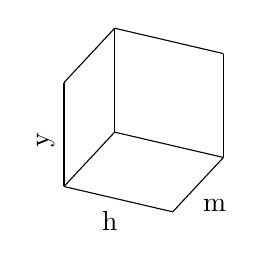
\begin{tikzpicture}
\begin{axis}[
    axis equal image=true,
    xlabel=h,
    ylabel=m,
    zlabel=y,
    xmin=0,
    xmax=1,
    ymin=0,
    ymax=1,
    zmin=0,
    zmax=1,
    ticks=none,
    axis lines=box,
    y dir=reverse,
    ylabel style={rotate=-90},
    height=5cm,
    ]
    \arrowo{0,1}
    \arrowk{1,0}
    \arrowx{0,1}
\end{axis}
\end{tikzpicture}
\hspace{0.5cm}
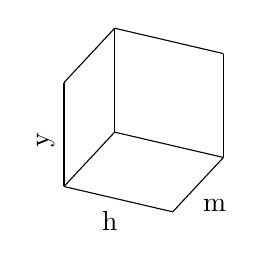
\begin{tikzpicture}
\begin{axis}[
    axis equal image=true,
    xlabel=h,
    ylabel=m,
    zlabel=y,
    xmin=0,
    xmax=1,
    ymin=0,
    ymax=1,
    zmin=0,
    zmax=1,
    ticks=none,
    axis lines=box,
    y dir=reverse,
    ylabel style={rotate=-90},
    height=5cm,
    ]
    \arrowo{1,0}
    \arrowk{1,0}
    \arrowx{1,1}
    \plane{1,0,0}{1,0,1}{0,0,1}
\end{axis}
\end{tikzpicture}
\hspace{0.5cm}
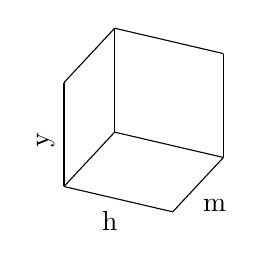
\begin{tikzpicture}
\begin{axis}[
    axis equal image=true,
    xlabel=h,
    ylabel=m,
    zlabel=y,
    xmin=0,
    xmax=1,
    ymin=0,
    ymax=1,
    zmin=0,
    zmax=1,
    ticks=none,
    axis lines=box,
    y dir=reverse,
    ylabel style={rotate=-90},
    height=5cm,
    ]
    \arrowo{1,0}
    \arrowkx{1,1}{1,1}
\end{axis}
\end{tikzpicture}
\caption{
Visual representation of the Matyas-Meyer-Oseas compression function (left) and two insecure compression functions (middle, right).
The arrows represent $\O$ (black), $\vk$ (red) and $\vx$ (blue).
A violet arrow means $\vk = \vx$.
One should keep in mind that $\rowsp(\C)$ includes the vector $\vy$, which is omitted as it always points up.
A gray plane is sometimes drawn to highlight the fact that $\C$ is deterministically solvable fixing $\rowsp(\O) + \rowsp(k)$.
}
\label{fig:graphical_rep}
\end{figure}

Let $\P = (\I, \O, \C)$ be the Linicrypt program corresponding to a scheme $f$ which insecure as a compression function
(condition \eqref{eq_compression_secure} does not hold).
This is equivalent to the statement:
$\P$ has a collision structure.
By definition of collision structure,
there is a split $\C = \Ccs \sqcup \Cfix$ such that $\Ccs$ is deterministically solvable fixing a space
\begin{equation}
\label{eq_coll_structure_compression_functions}
\Fix \supsetneq \rowsp(\Cfix) + \rowsp(\O).
\end{equation}
As $\C = \{(\vk, \vx, \vy)\}$ contains only a single element,
there are only two cases for this split.

\textbf{Case 1: $\Ccs = \{\}$ and $\Cfix = \C$.}

In this case, we know by definition that $\Fix$ has to be the whole space $\Frowsp$.
Therefore, equation \ref{eq_coll_structure_compression_functions} translates to
$\rowsp(\O, \vk, \vx, \vy) \neq \Fix = \Frowsp$.
This is exactly the condition by which the authors of \cite{TCC:McQSwoRos19} call $\P$ degenerate.

\begin{defn}
    Let $f$ be one of the 64 PGV compression functions.
    We assign it to the Linicrypt attack category ``Degenerate" if $\rowsp(\O,\vk,\vx,\vy) \neq \Frowsp$.
\end{defn}

\begin{lemma}(Degenerate Attack)
    Let $f$ be a compression scheme from the Degenerate category.
    Then there is a second preimage attack on $H^n_f$ if $n>1$.
    There are 22 such compression schemes.
\end{lemma}
\begin{proof}
Let $(m_1, \dots, m_n)$ be an input for $H^n_f$.
We will describe how to find a second-preimage for it.
Note, that 
\[
\rowsp(\O, \vk, \vx, \vy)\t = \ker(\O)^\perp + \ker(\C)^\perp = \big(\ker(\O) \cap \ker(\C)\big)^\perp.
\] 
Recall, that the space $\ker(\O) \cap \ker(\C)$ carries the following meaning:
Let $\vw \in \ker(\O) \cap \ker(\C)$ be arbitrary.
If $\vv$ is in $\sol(\C)$ then $\vv + \vw$ is in $\sol(\C)$ with $\O\vv = \O(\vv + \vw)$.
In other words: $\P\big(\I(\vv + \vw)\big) = \O(\vv + \vw) = \O\vv = \P(\I\vv)$.

As $f$ is degenerate, $\dim\big(\rowsp(\O,\vk,\vx,\vy)\big) \leq 2$.
Also, $\vy = \ve^3 \in \rowsp(\O, \vk, \vx, \vy)$.
Therefore, $\ker(\O) \cap \ker(\C)$ can only be one of 4 subspaces.
We do a case separation for these 4 subspaces.

% \textbf{Case 1.1: $\ker(\O) \cap \ker(\C) = \spn(\ve_1, \ve_2) = \rowsp(\vh)\t + \rowsp(\vm)\t = \spn(\vh\t, \vm\t)$.}
\textbf{Case 1.1: $\ker(\O) \cap \ker(\C) = \rowsp(\vh, \vm)\t = \spn(\ve_1, \ve_2)$.}

It follows that $\rowsp(\C) = \rowsp(\O) = \rowsp(\ve_3)$, i.e. $\vk = \vx = 0$ and $\O = \ve^3$.
This is the scheme $f(h,m) = E(0,0)$.
The function $H^n_f$ is constant, so every input is a collision with every other input.
This is the graphical representation of its algebraic representation.
\begin{center}
\centering
\cube{\arrowo{0,0}\arrowkx{0,0}{0,0}}
\end{center}

\textbf{Case 1.2: $\ker(\O) \cap \ker(\C) = \rowsp(\vm)\t = \spn(\ve_2)$.}

Let $\m{0&\delta&0} \in \ker(\O) \cap \ker(\C)$ be arbitrary.
By the argument above, we have $f(h,m) = f(h,m + \delta)$ for any $h, m \in \F$.
We set $m_i' = m_i$ for $i<n$ and choose an $m_n' \neq m_n$.
Then 
\[
H^n_f(m_1', \dots, m_n') = h_n' = f(h_{n-1}, m_n') = f(h_{n-1}, m_n) = h_n = H^n_f(m_1, \dots, m_n).
\]
There are $2 \times 3 + 1 = 7$ compression schemes that fulfill the condition from his case.
\begin{center}
\cube{\arrowo{0,0}\arrowkx{0,1}{0,1}}
\cube{\arrowo{0,0}\arrowkx{0,1}{0,0}}
\cube{\arrowo{0,0}\arrowkx{0,0}{0,1}}
\cube{\arrowo{0,1}\arrowkx{0,1}{0,1}}
\cube{\arrowo{0,1}\arrowkx{0,1}{0,0}}
\cube{\arrowo{0,1}\arrowkx{0,0}{0,1}}
\cube{\arrowo{0,1}\arrowkx{0,0}{0,0}}
\end{center}

\textbf{Case 1.3: $\ker(\O) \cap \ker(\C) = \rowsp(\vh)\t = \spn(\ve_1)$.}

By the same argument as in the previous case, we get $f(h,m) = f(h',m)$ for any $h' \in \F$.
We set $m_i' = m_i$ for $i<n-1$, $m_{n-1}' \neq m_{n-1}$ and $m_n' = m_n$. 
Then
\[
H^n_f(m_1', \dots, m_n') = h_n' = f(h_{n-1}', m_n) = f(h_{n-1}, m_n) = h_n = H^n_f(m_1, \dots, m_n).
\]
There are $2 \times 3 + 1 = 7$ compression schemes that fulfill the condition from his case.
\begin{center}
\cube{\arrowo{0,0}\arrowkx{1,0}{1,0}}
\cube{\arrowo{0,0}\arrowkx{1,0}{0,0}}
\cube{\arrowo{0,0}\arrowkx{0,0}{1,0}}
\cube{\arrowo{1,0}\arrowkx{1,0}{1,0}}
\cube{\arrowo{1,0}\arrowkx{1,0}{0,0}}
\cube{\arrowo{1,0}\arrowkx{0,0}{1,0}}
\cube{\arrowo{1,0}\arrowkx{0,0}{0,0}}
\end{center}

\textbf{Case 1.4: $\ker(\O) \cap \ker(\C) = \rowsp(\vh - \vm)\t = \spn(\ve_1 - \ve_2)$.}

This implies that $f(h,m) = f(h + \delta, h - \delta)$ for any $\delta \in \F$.
We set $m_i' = m_i$ for $i<n-1$, $m_{n-1}' \neq m_{n-1}$, $\delta = h_{n-1} - h_{n-1}'$ and $m_n' = m_n + \delta$.
Then
\[
h_n' = f(h_{n-1}', m_n') = f(h_{n-1}' + \delta, m_n' - \delta) = f(h_{n-1}, m_n) = h_n.
\]
There are $2 \times 3 + 1 = 7$ compression schemes that fulfill the condition from his case.
\begin{center}
\cube{\arrowo{0,0}\arrowkx{1,1}{1,1}}
\cube{\arrowo{0,0}\arrowkx{1,1}{0,0}}
\cube{\arrowo{0,0}\arrowkx{0,0}{1,1}}
\cube{\arrowo{1,1}\arrowkx{1,1}{1,1}}
\cube{\arrowo{1,1}\arrowkx{1,1}{0,0}}
\cube{\arrowo{1,1}\arrowkx{0,0}{1,1}}
\cube{\arrowo{1,1}\arrowkx{0,0}{0,0}}
\end{center}

In total found $1 + 3\times7 = 22$ degenerate compression schemes.
This completes the proof.
\end{proof}

This completes the analysis of case 1.
Now consider the other split of $\C$ into $\Ccs \sqcup \Cfix$.

\textbf{Case 2: $\Ccs = \C$ and $\Cfix = \{\}$.}

By the assumption that $f$ has a collision structure, we get:
$\C$ is deterministically solvable fixing $\Fix \supsetneq \rowsp(\O)$.
Recall, that this means one can fix $\O\vv$ and some other base variables value arbitrarily and still find a $\vv \in \sol(\C)$.
$\Fix$ has to be 2 dimensional, because of the bijection from the inputs of a program to $\sol(\C)$.
The 2-dimensional subspace $\Fix$ can only be one of these 7.
\begin{center}
\cubealt{\plane{1,0,0}{1,0,1}{0,0,1}}
\cubealt{\plane{1,1,0}{1,1,1}{0,0,1}}
\cubealt{\plane{0,1,0}{0,1,1}{0,0,1}}
\cubealt{\plane{1,1,0}{1,0.5,0.5}{1,0,1}}
\cubealt{\plane{0,1,0}{1,1,1}{1,0,1}}
\cubealt{\plane{1,0,0}{1,1,1}{0,1,1}}
\cubealt{\plane{1,1,0}{0.5,1,0.5}{0,1,1}}
\end{center}
In the case that $\vh \in \Fix$ a second preimage attack is possible.
Only the first and the 5th subspace pictured above fulfill this condition.

\textbf{Case 2.1: $\C$ is deterministically solvable fixing $\O$ and $\vh$.}

\begin{defn}
    Let $f$ be one of the 64 PGV compression functions with algebraic representation $(\I, \O, \C)$.
    We assign it to the Linicrypt attack category ``$\<\O, \vh\>$-Collision Structure" if
    $\C$ is deterministically solvable fixing $\O$ and $\vh$.
\end{defn}

\begin{lemma}
    Let $f$ be a compression scheme from the $\<\O, \vh\>$-Collision Structure category.
    Then there is a second-preimage attack on $H^n_f$ making a single query to the ideal cipher.
    Also, its attack type is (b) in \cite{C:BlaRogShr02} and (D) in \cite{C:PreGovVan93}.
    There are 12 such compression schemes.
\end{lemma}

\begin{proof}
    Assume we are given any $o, h \in \F$.
    We show that a corresponding $m \in \F$ can be found such that $f(h,m) = o$.
    This is the definition of the direct attack (D) from \cite{C:PreGovVan93} which corresponds to attack (b) from \cite{C:BlaRogShr02}.
    Assume as stated in the Lemma: $\C$ is deterministically solvable fixing $\Ics = \m{\O \\ \vh}$.

    By Lemma \ref{lemma:solution_space_bijection_ic}, $\Ics|_{\sol(\C)} : \sol(\C) \to \F^2$ is a bijection.
    Corollary \ref{corollary:det_solvable_computeable_ic} states that the preimage to $(o,h)$ can be computed using $|\C| = 1$ queries.
    We call this preimage $\vv \in \sol(\C)$.
    By definition of $\Ics$ we have $\O\vv = o$ and $\vh\vv = h$.
    We set $m = \vm \vv$.
    Then $f(h,m) = f(\vh\vv, \vm\vv) = \O\vv = o$ as required.
    
    This allows for an easy second-preimage attack on $H^n_f$.
    Let $(m_1, \dots, m_n)$ be an input to $H^n_f$.
    We set $m_i' = m_i$ for $i<n-1$ and $m_{n-1}' \neq m_{n-1}$.
    According to the argument above, we can compute an $m_n'$, such that
    \[
    H^n_f(m_1', \dots, m_n') = h_n' = f(h_{n-1}', m_n') = h_n = H^n_f(m_1, \dots, m_n).
    \]

We will now list and count the schemes described by the Lemma.
First, note that $\vk \in \spn(\O, \vh)$ by definition of deterministically solvable.
Therefore, $\vk = 0$ or $\vk = \vh$.
We can derive these two implications:
\begin{align}
\vk \neq 0 &\implies \C \textrm{ deterministically solvable fixing } \O, \vk \\
\vk = 0    &\implies \C \textrm{ deterministically solvable fixing } \O, \vy \textrm{ or fixing } \O, \vx
\end{align}

Assume $\rowsp(\O, \vh) = \rowsp(\vy, \vh)$.
Then these 6 schemes correspond to this subcase:

\begin{center}
\cube{\plane{1,0,0}{1,0,1}{0,0,1}\arrows{0,0}{1,0}{0,1}}
\cube{\plane{1,0,0}{1,0,1}{0,0,1}\arrows{0,0}{1,0}{1,1}}
\cube{\plane{1,0,0}{1,0,1}{0,0,1}\arrows{1,0}{1,0}{0,1}}
\cube{\plane{1,0,0}{1,0,1}{0,0,1}\arrows{1,0}{1,0}{1,1}}
\cube{\plane{1,0,0}{1,0,1}{0,0,1}\arrows{1,0}{0,0}{0,1}}
\cube{\plane{1,0,0}{1,0,1}{0,0,1}\arrows{1,0}{0,0}{1,1}}
\end{center}
Now assume $\rowsp(\O, \vh) = \rowsp(\vy + \vm, \vh)$.
Then these 6 schemes correspond to this subcase:

\begin{center}
\cube{\plane{1,0,0}{1,1,1}{0,1,1}\arrows{0,1}{1,0}{1,0}}
\cube{\plane{1,0,0}{1,1,1}{0,1,1}\arrows{0,1}{1,0}{0,0}}
\cube{\plane{1,0,0}{1,1,1}{0,1,1}\arrows{0,1}{0,0}{1,0}}
\cube{\plane{1,0,0}{1,1,1}{0,1,1}\arrows{1,1}{1,0}{1,0}}
\cube{\plane{1,0,0}{1,1,1}{0,1,1}\arrows{1,1}{1,0}{0,0}}
\cube{\plane{1,0,0}{1,1,1}{0,1,1}\arrows{1,1}{0,0}{1,0}}
\end{center}
Altogether these are 12 compression schemes.
\end{proof}


At this point, out of the 42 schemes with a collision structure, 18 are left.
Unfortunately, the categorization of these does not follow directly from the Linicrypt model as the first two categories do.
This is because the attacks on them rely on causing interactions between different queries.
Neither our security proof, which is restricted to single query constructions
nor the proof from \cite[Theorem 1]{TCC:McQSwoRos19}, which is restricted to constructions using distinct nonces,
can explain these behaviors.

Consider the Permutation Attack from \cite{C:PreGovVan93}.
It can be described by the following condition on the algebraic representation of $f$.

\textbf{Case 2.2: $\vh\t \in \ker(\C)$.}

This case overlaps with both Case 1 and Case 2.1.
$\vh\t \in \ker(\C)$ equivalent to setting the parameters $c$ and $e$ to 0.
That is, $f(h,m) = ah + f_2(m)$ for some function $f_2$ and $a \in \{0,1\}$.
Then 
\[
H^n_f(\dts m n) = f(h_{n-1}, m_n) = a h_{n-1} + f_2(m_n) = \cdots = a^n h_{0} + \sum_{i=1}^n a^{n-i}f_2(m_i).
\]
Therefore, $H^n_f(m_0, \dots, m_n) = H^n_f(m_{\pi(0)}, \dots, m_{\pi(0)})$ for a permutation $\pi$ of $\{1, \dots, n\}$.
If $n \geq 1$ this allows for a second preimage attack which does not need any queries to the ideal cipher.
One can identify $2^{6-2} = 16$ schemes $f$ such that $H^n_f$ is susceptible to this permutation attack.
The 5 schemes that meet this requirement and have not yet been categorized are:
\begin{center}
\cubealt{\plane{0,1,0}{1,1,1}{1,0,1}\arrows{1,0}{0,1}{0,1}}
\cubealt{\plane{0,1,0}{1,1,1}{1,0,1}\arrows{1,0}{0,1}{0,0}}
\cubealt{\plane{0,1,0}{1,1,1}{1,0,1}\arrows{1,1}{0,1}{0,1}}
\cubealt{\plane{0,1,0}{1,1,1}{1,0,1}\arrows{1,1}{0,0}{0,1}}
\cubealt{\plane{0,1,0}{1,1,1}{1,0,1}\arrows{1,1}{0,1}{0,0}}
\end{center}

\textbf{Case 2.3: None of the above cases.}

Finally, we are left with 13 schemes.
These are exactly the 13 schemes of the type Backward Attack (B) from \cite{C:PreGovVan93}.
8 of those schemes have been shown to be secure if composed in the \MD construction by \cite{C:BlaRogShr02}.
They call them the group-2 schemes with attack type (c).
This is the visual representation corresponding to them:
\begin{center}
\cube{\plane{1,1,0}{1,1,1}{0,0,1}\arrows{0,0}{1,1}{0,1}}
\cube{\plane{1,1,0}{1,1,1}{0,0,1}\arrows{0,0}{1,1}{1,0}}
\cube{\plane{1,1,0}{1,1,1}{0,0,1}\arrows{1,1}{1,1}{1,0}}
\cube{\plane{1,1,0}{1,1,1}{0,0,1}\arrows{1,1}{1,1}{0,1}}
\cube{\plane{0,1,0}{0,1,1}{0,0,1}\arrows{0,0}{0,1}{1,0}}
\cube{\plane{0,1,0}{0,1,1}{0,0,1}\arrows{0,0}{0,1}{1,1}}
\cube{\plane{0,1,0}{0,1,1}{0,0,1}\arrows{0,1}{0,1}{1,0}}
\cube{\plane{0,1,0}{0,1,1}{0,0,1}\arrows{0,1}{0,1}{1,1}}
\end{center}


The 5 remaining schemes are marked with attack type (g).
That means, that the authors \cite{C:BlaRogShr02} identified a collision attack making 2 or fewer queries.
These collisions are special, as they can be produced only for different input lengths.
Take for example the compression scheme $f(h,m) = \E(0,h+m) + m$.
Let $n$ be fixed.
For $i \leq n$ we define the message blocks:
\[
m_i = \begin{cases}
0 & \textrm{for odd $i$} \\
-E(0,0) & \textrm{for even $i$}
\end{cases}
\]
Then the Linicrypt \MD construction computes to:
\[
H_f^n(m_1, \dots, m_n) = \begin{cases}
E(0,0) & \textrm{for odd $n$} \\
0 & \textrm{for even $n$}
\end{cases}
\]
All the collisions we found are then: $H^n_f(m_1, \dots, m_n) = H^{n-2}_f(m_1, \dots, m_{n-2})$.

For the two schemes where $\O = \m{1&0&1}$ the collisions are very similar in structure,
if one assumes the field $\F$ has characteristic 2, i.e. $x + x = 0$ for any $x \in \F$.

\begin{center}
\cubealt{\plane{1,1,0}{1,0.5,0.5}{1,0,1}\arrows{1,0}{1,1}{1,1}}
\cubealt{\plane{1,1,0}{1,0.5,0.5}{1,0,1}\arrows{1,0}{1,1}{0,0}}
\cubealt{\plane{1,1,0}{0.5,1,0.5}{0,1,1}\arrows{0,1}{1,1}{1,1}}
\cubealt{\plane{1,1,0}{0.5,1,0.5}{0,1,1}\arrows{0,1}{1,1}{0,0}}
\cubealt{\plane{1,1,0}{0.5,1,0.5}{0,1,1}\arrows{0,1}{0,0}{1,1}}
\end{center}

To conclude this section we have summarized the comparison of the Linicrypt attack taxonomy and the previous taxonomies in Table \ref{table:64_compression_schemes}.
From the derivation, it is clear that the subspaces for which $\C$ is deterministically solvable
contain a lot of information about the security properties of the scheme.

\begin{table}[ht]
\centering
\renewcommand{\arraystretch}{1.2}
\begin{tabular}{lllrc}
\toprule
 &  &  & \# & $\spradv(\A, \H^n_f)$ \\
Linicrypt Attack & BRS & PGV &  &  \\
\midrule
\multirow[c]{3}{*}{Degenerate} & a & - & 15 & 1 \\
\cline{2-5} \cline{3-5}
 & b & D & 2 & 1 \\
\cline{2-5} \cline{3-5}
 & g & F & 5 & 1 \\
\cline{1-5} \cline{2-5} \cline{3-5}
$\<\O, \vh\>$-Collision Structure & b & D & 12 & 1 \\
\cline{1-5} \cline{2-5} \cline{3-5}
Permutation attack & f & P & 5 & 1 \\
\cline{1-5} \cline{2-5} \cline{3-5}
\multirow[c]{2}{*}{Secure} & d & $\checkmark$ & 4 & $\leq N/|\F|$ \\
\cline{2-5} \cline{3-5}
 & e & FP & 8 & $\leq N/|\F|$ \\
\cline{1-5} \cline{2-5} \cline{3-5}
\multirow[c]{2}{*}{Other Collision Structure} & c & B & 8 &  \\
\cline{2-5} \cline{3-5}
 & g & B & 5 &  \\
\cline{1-5} \cline{2-5} \cline{3-5}
\bottomrule
\end{tabular}

\caption{
    Comparison of the classification derived by the Linicrypt model and the ones found by \cite{C:PreGovVan93} and \cite{C:BlaRogShr02}.
    The $f$ in $\PMD{f}$ stands for the associated function to one of the compression schemes in that row.
    The $\A$ denotes the best possible adversary.
    This table, including the Linicrypt attack type, has been generated automatically.
    The code is accessible in \cite{Semmel_Code_for_Modeling_2022}.
    }
\label{table:64_compression_schemes}
\end{table}

